\section{Antecedentes del recinto}
\noindent 
El Centro de Extensión Campus Los Canelos de la Universidad Austral de Chile, ubicado en la calle Yerbas Buenas, en la ciudad de Valdivia, inaugurado en $2019$, busca ``acoger y congregar a diferentes comunidades en torno a las artes, las culturas, la extensión científica, temas públicos e iniciativas del área de la salud. Atendiendo a los lineamientos y políticas de vinculación con el medio universitarias se priorizó la adecuación de los espacios con una orientación hacia su uso público. Este centro cuenta con tres salones multiuso para exposiciones, charlas y conferencias, sumando más de $250$ $m^2$ de superficie totalmente equipados con sistemas de audio y video. Además, alberga a las distintas unidades, programas y áreas que conforman la Dirección de Vinculación con el medio, con un espacio cercano a los $300$ $m^2$ utilizados como salas de reuniones y oficinas.'' \cite{loscanelos}

\begin{figure}[H]
    \centering
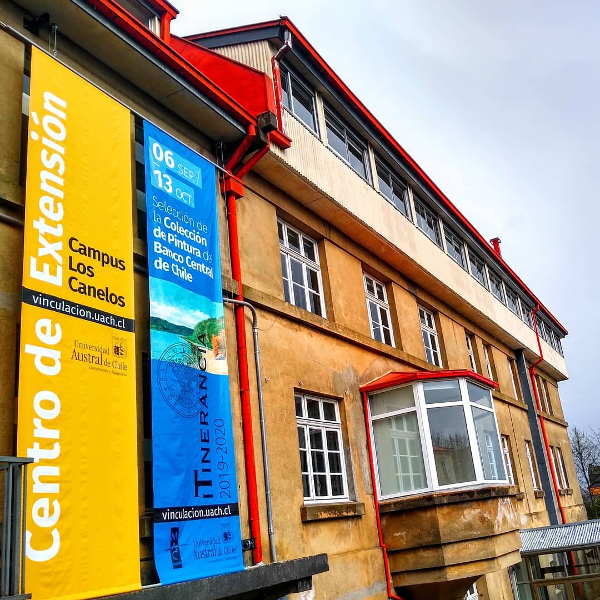
\includegraphics[scale=0.45]{Imagenes/centroextensionuach.jpg}
    \caption{Centro de Extensión Campus los Canelos, UACh.}
    \label{fig:los-canelos}
\end{figure}

\noindent En específico, este proyecto considera el acondicionamiento acústico de dos salas de reuniones, de $30$ y $35$ $m^2$, y la sala de ensayo de la Orquesta de Cámara de Valdivia, de $62$ $m^2$.

\noindent El Centro de Extensión Campus Los Canelos de la Universidad Austral de Chile, como se puede observar en la figura \ref{fig:geolocalización} se encuentra ubicado en Yerbas Buenas $181$, en la ciudad de Valdivia.
\begin{figure}[H]
    \centering
    \includegraphics[scale=0.5]{Imagenes/Antecedentes/Geolocalización.png}
    \caption{Geolocalización del edificio}
    \label{fig:geolocalización}
\end{figure}

\noindent Los salones a estudiar dentro del recinto son dos salas de reuniones con soporte para videoconferencia y una sala de ensayo utilizada por la Orquesta de Cámara de Valdivia, como se puede observar en las Figuras \ref{fig: foto sala1}, \ref{fig: foto sala2} y \ref{fig: foto sala OCV} respectivamente.
%insertar imagenes de recintos
\begin{figure}[H]
    \centering
    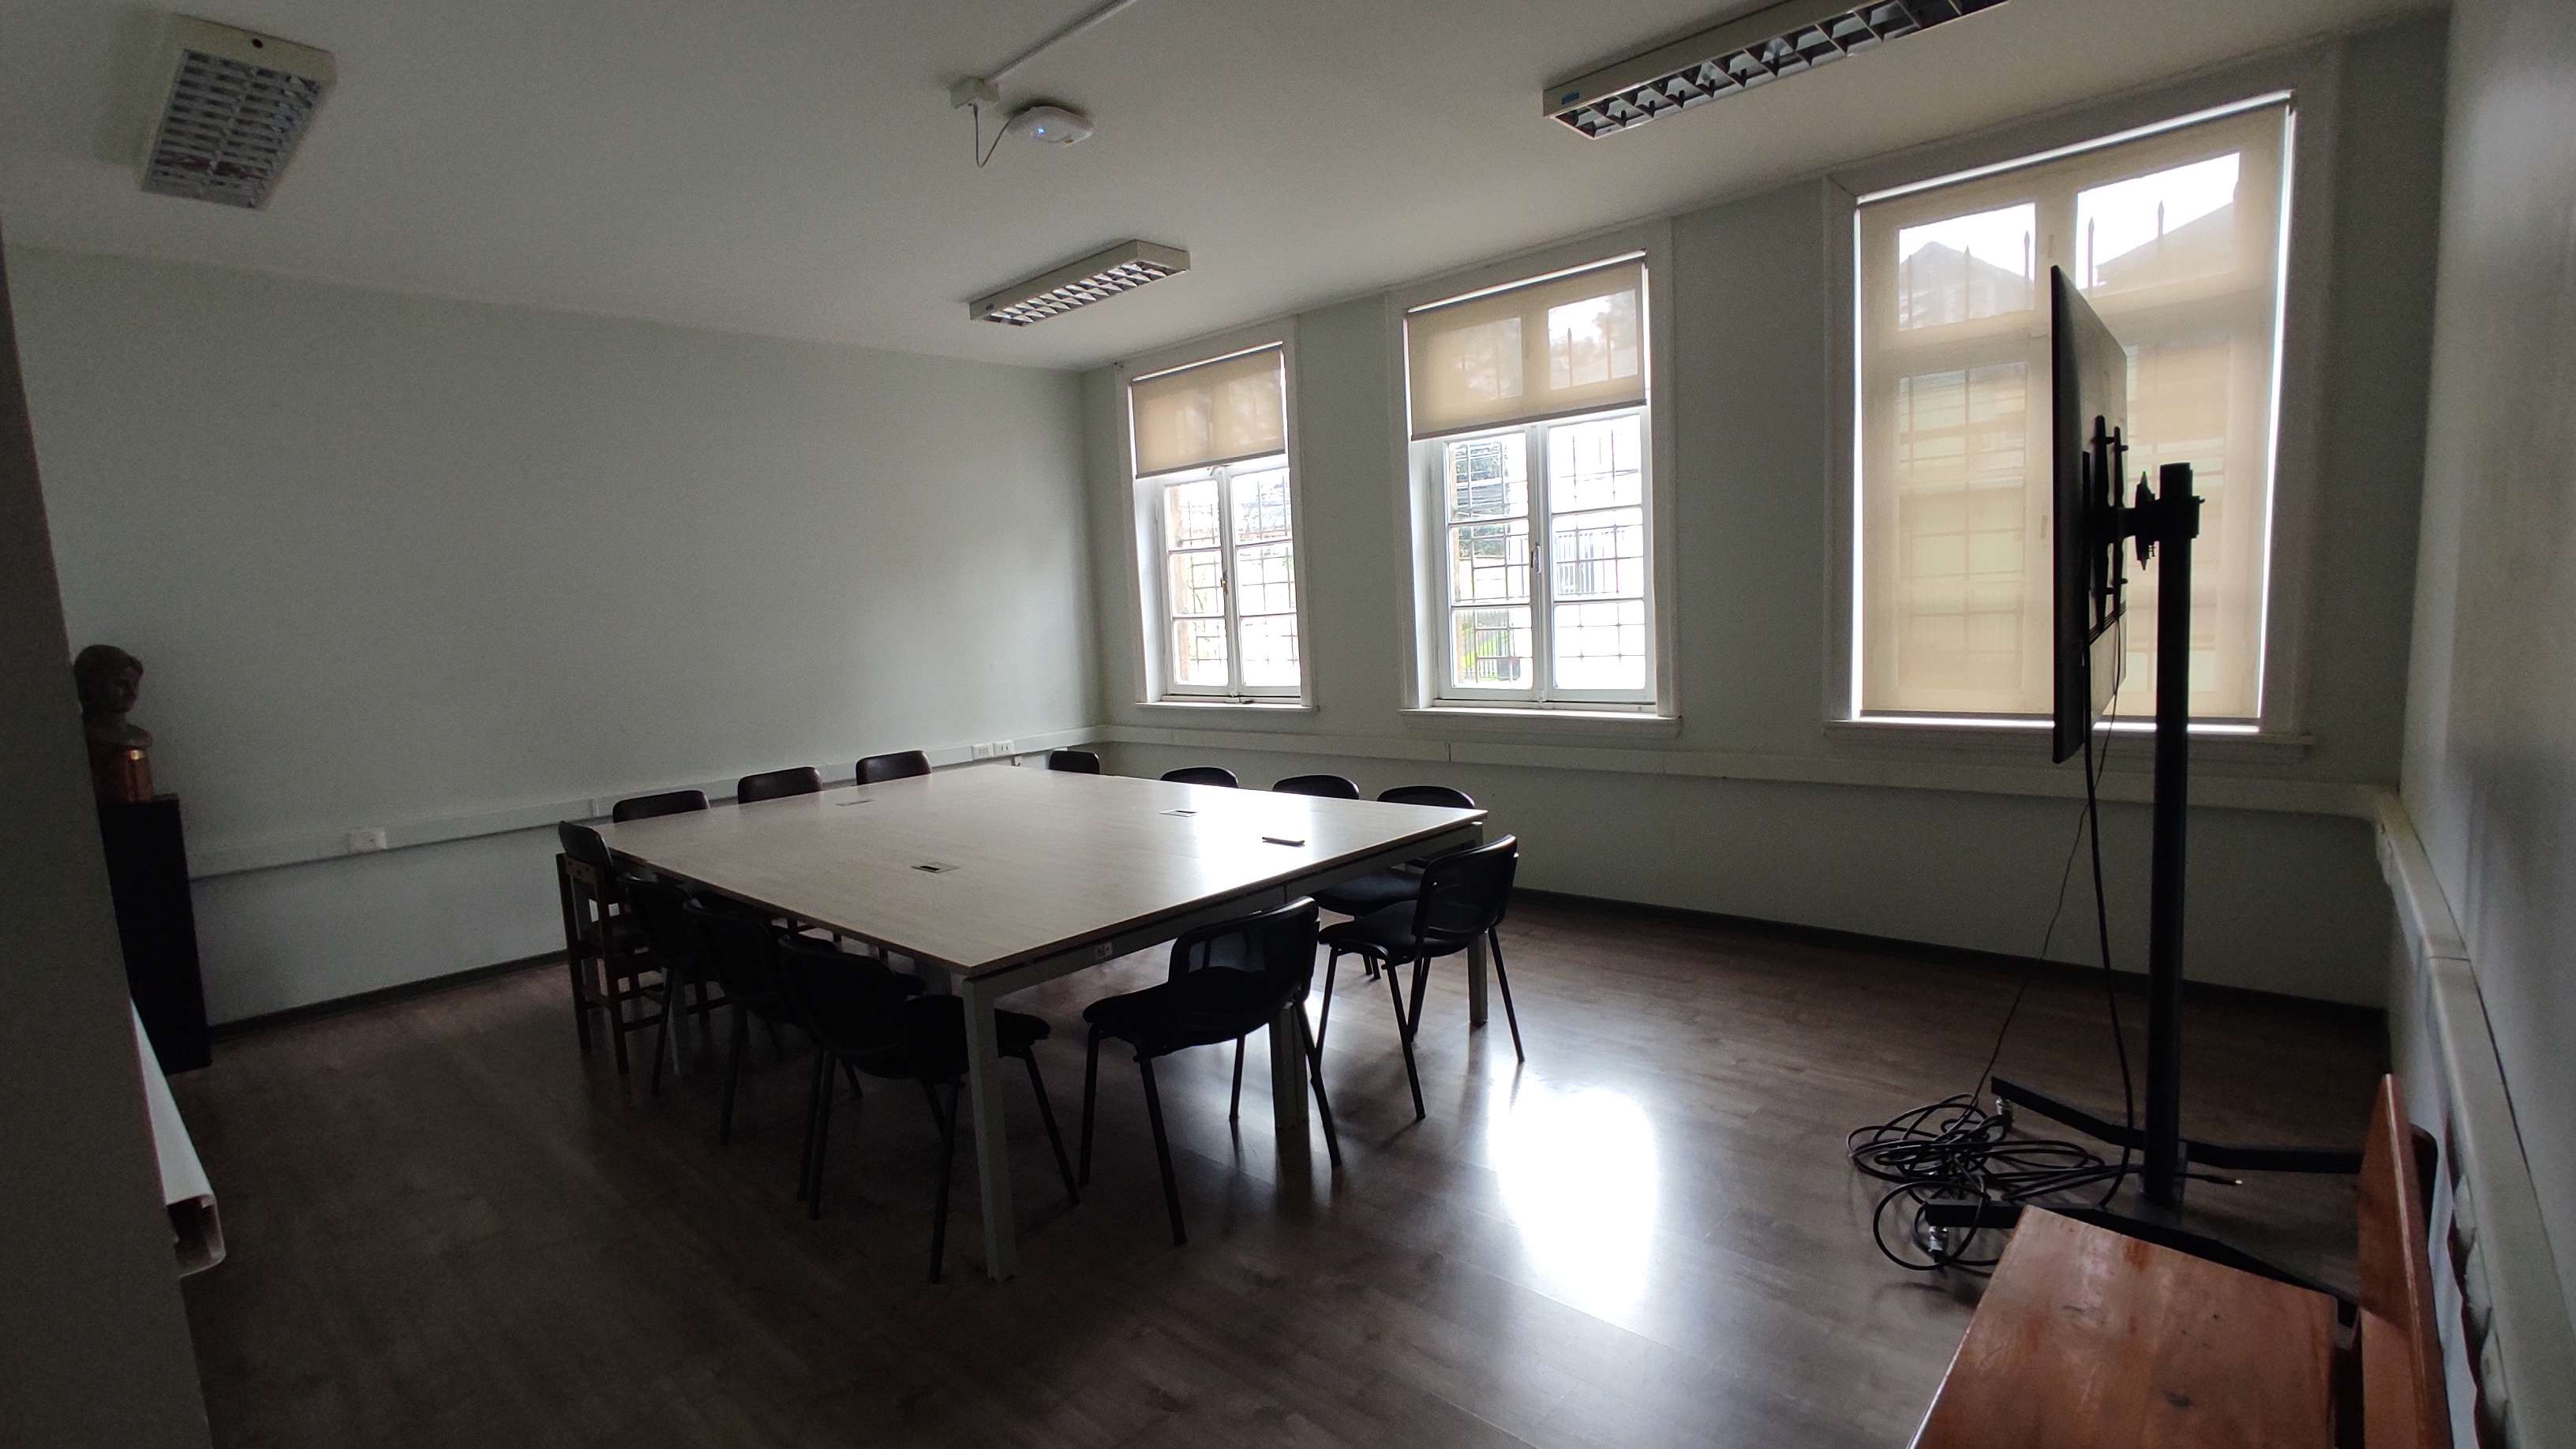
\includegraphics[scale=0.1]{Imagenes/Antecedentes/Sala 1.jpg}
    \caption{Fotografía de sala de reunión 1}
    \label{fig: foto sala1}
\end{figure}

\begin{figure}[H]
    \centering
    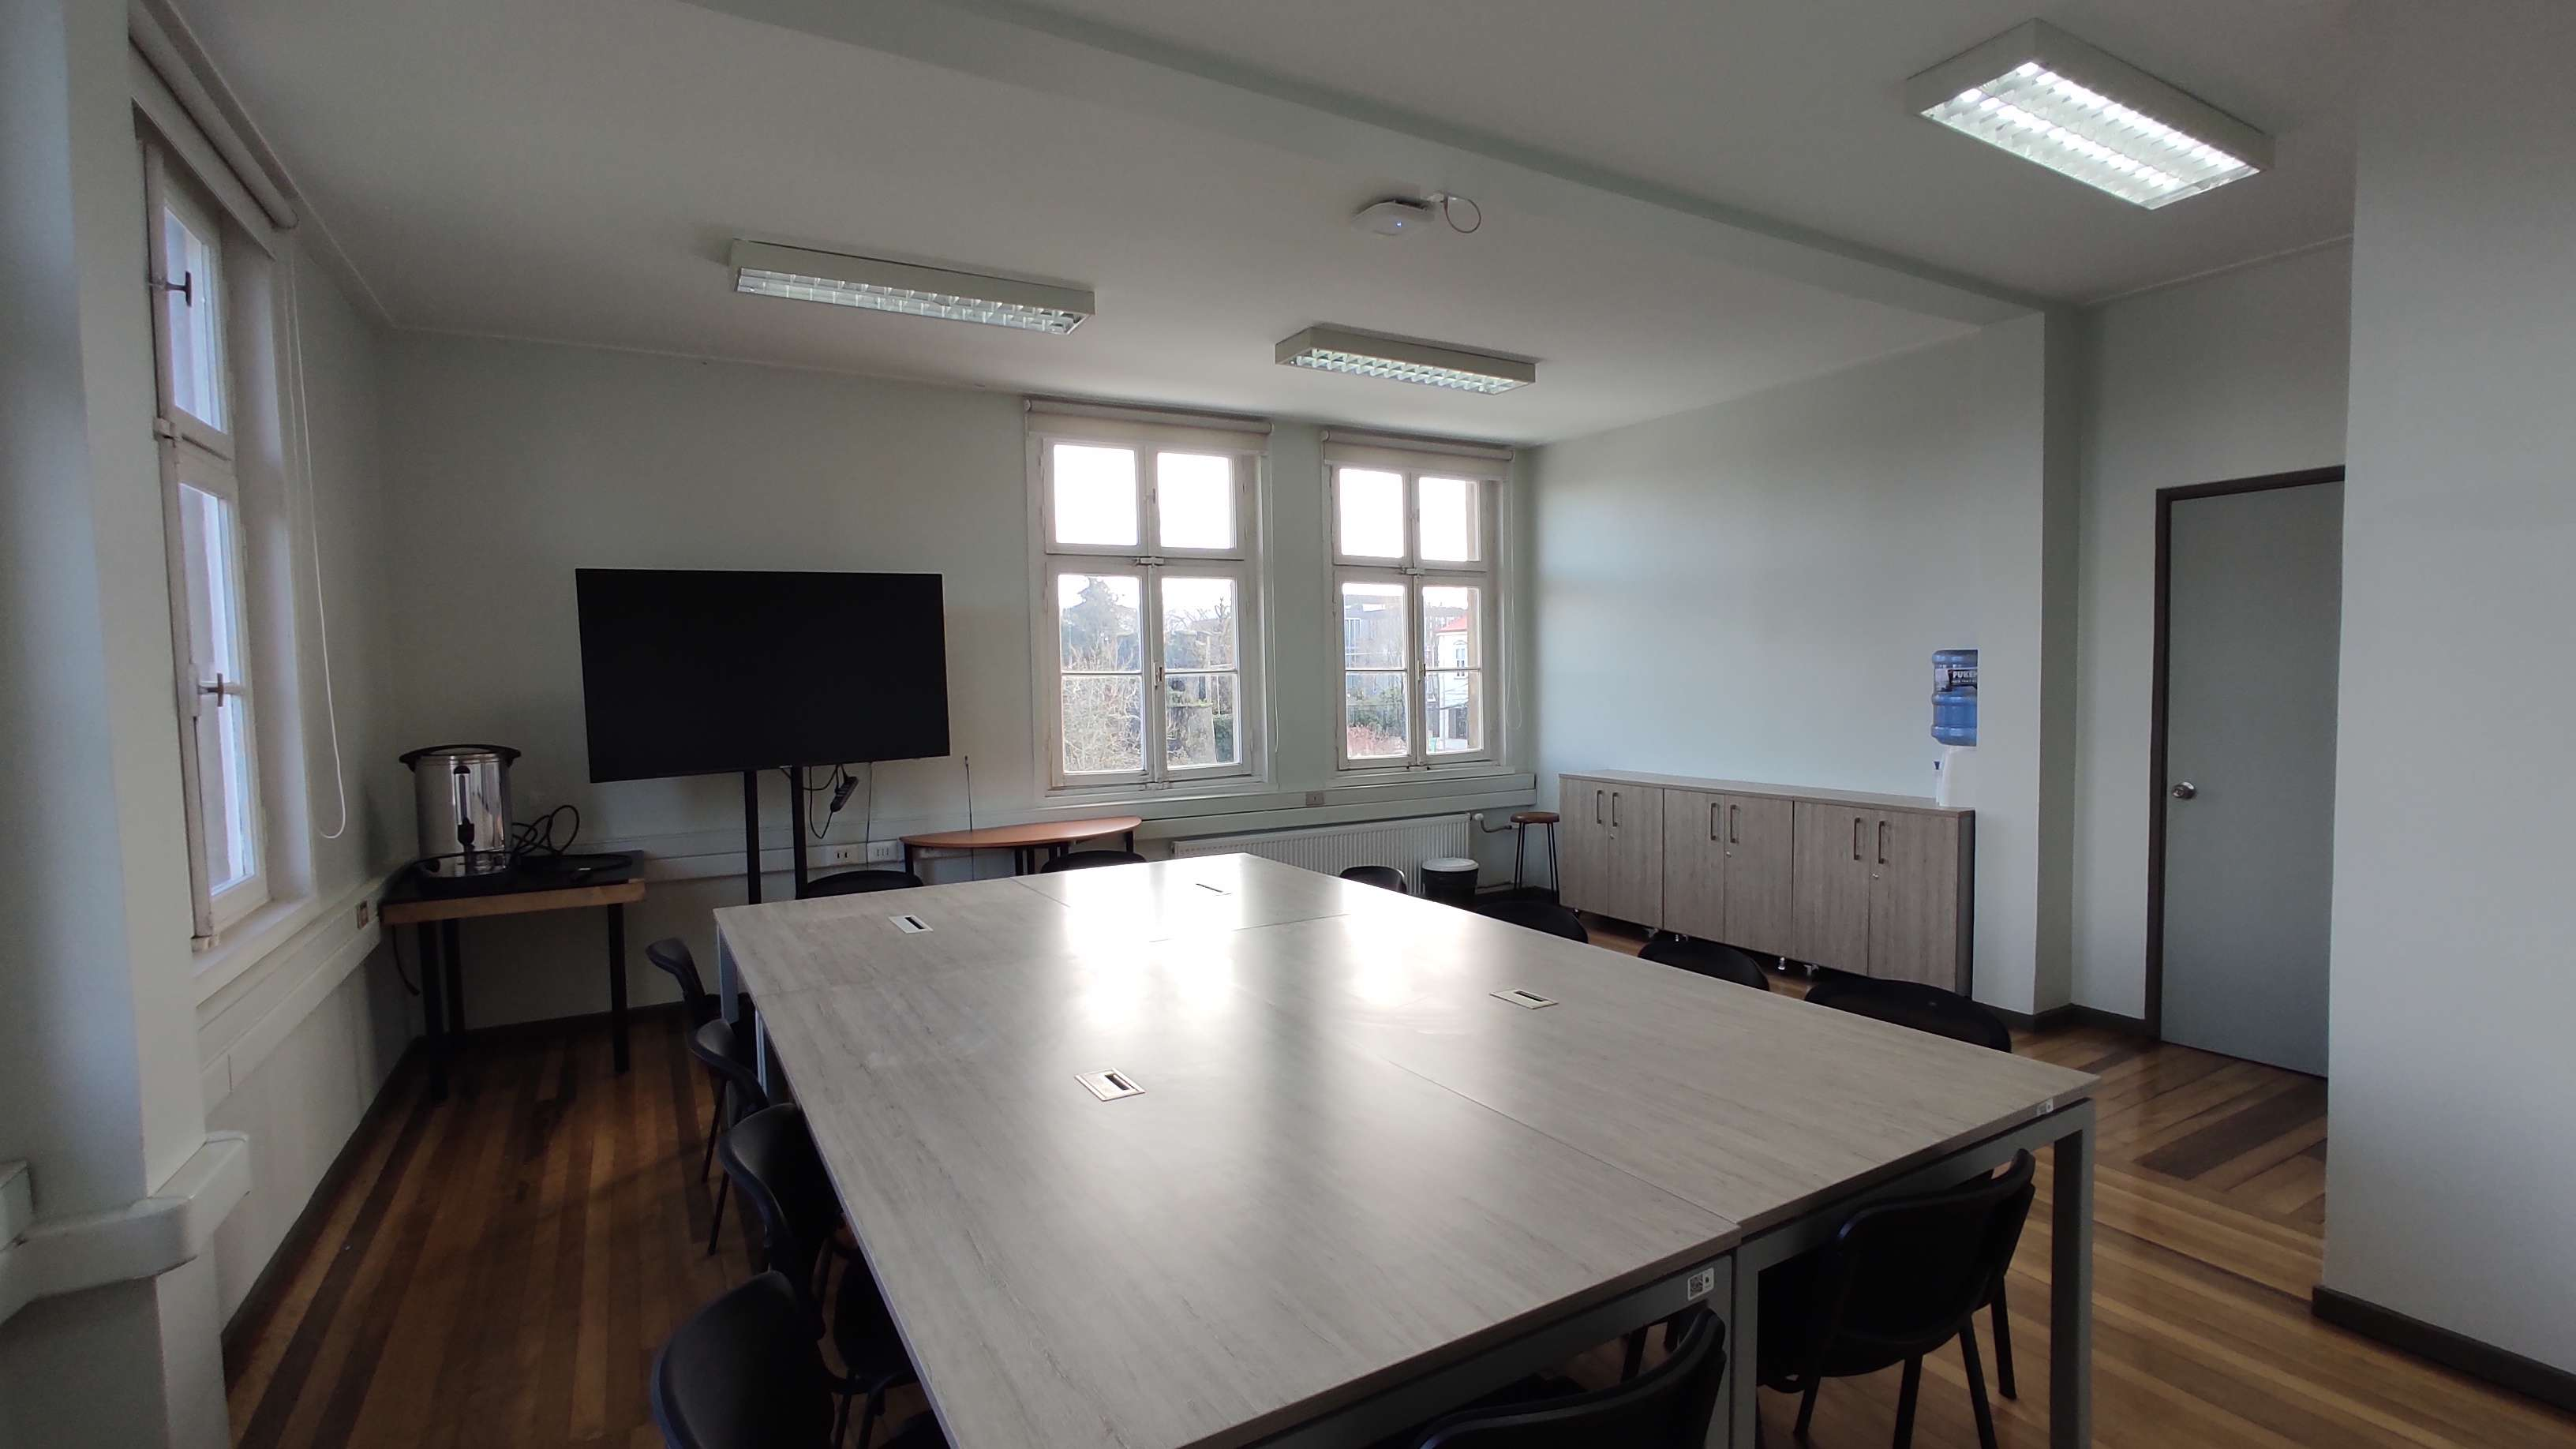
\includegraphics[scale=0.1]{Imagenes/Antecedentes/Sala 2.jpg}
    \caption{Fotografía de sala de reunión 2}
    \label{fig: foto sala2}
\end{figure}

\begin{figure}[H]
    \centering
    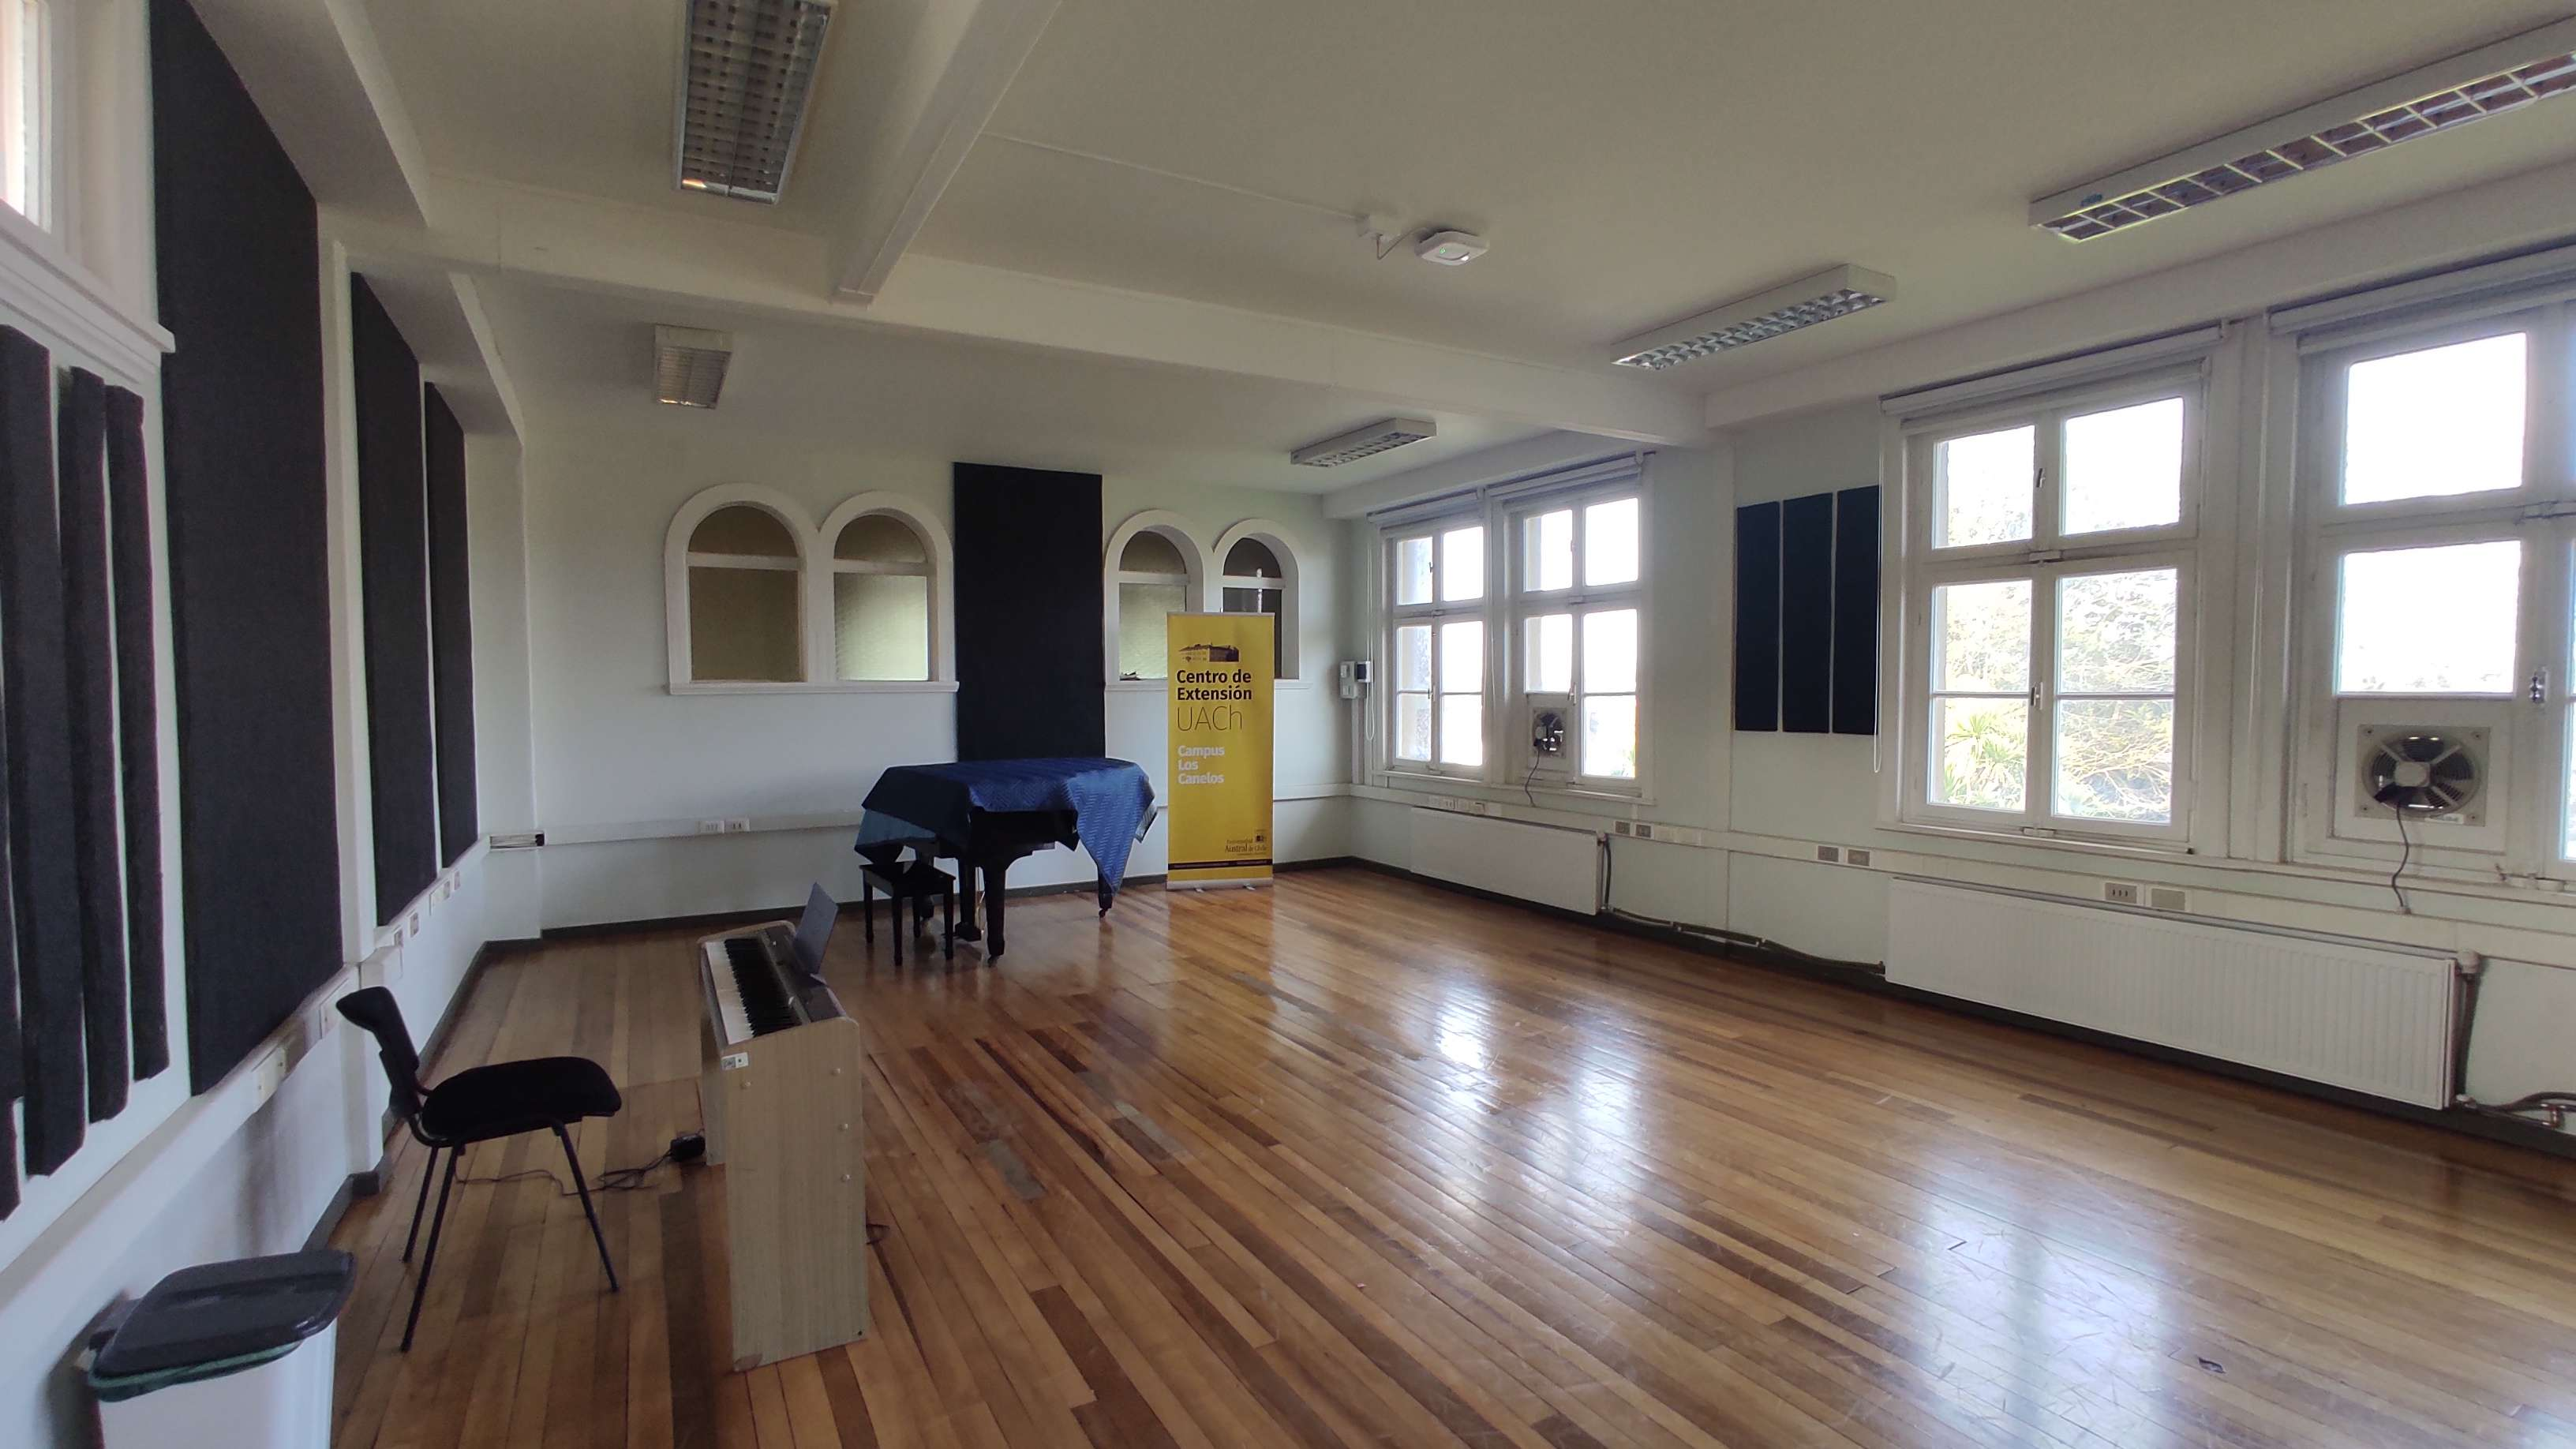
\includegraphics[scale=0.1]{Imagenes/Antecedentes/Sala OCV.jpg}
    \caption{Fotografía de sala de ensayo}
    \label{fig: foto sala OCV}
\end{figure}
